\chapter{Metodología}
\label{chap:metodologia}

 De acuerdo a \cite{Barrett2009}, el modelo WCM...\\

\subsection{M\'etodo de Osweiler}
copiar y pegar de la notebook.

\subsection{Tratamiento sobre Datos de Misi\'on}
En esta etapa repetimos el m\'etodo que propone Osweiler considerando los datos de misi\'on generados por el CODS
como posici\'on verdadera. 

\begin{figure}[!h]
 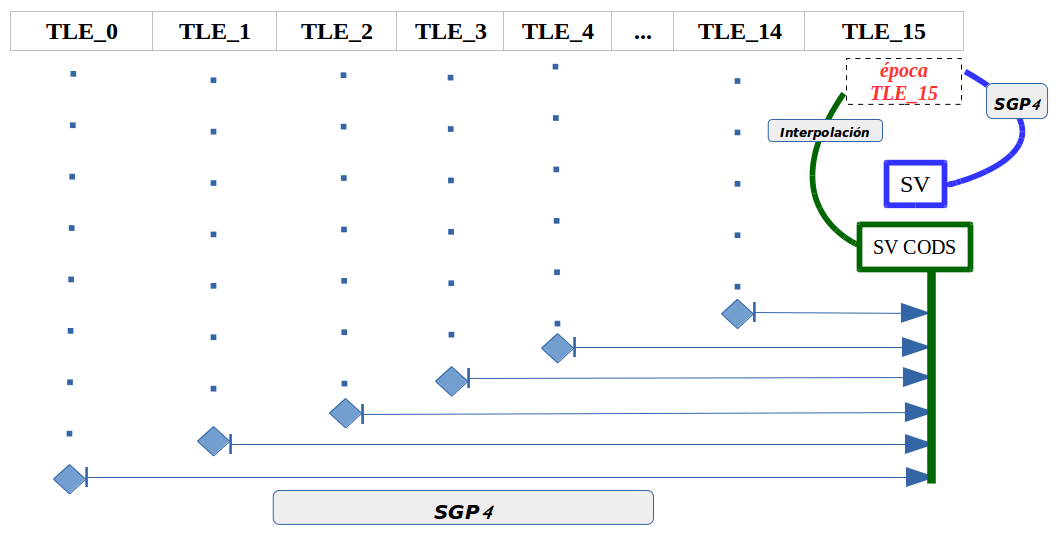
\includegraphics[width=0.7\textwidth]{imagenes/Osweiler_sobre_Cods.png}
 \caption{M\'etodo de Osweiler sobre datos CODS}
\end{figure}

Im\'agenes comparativas entre los dos m\'etodos:\\

\begin{figure}[H]
 \centering
\begin{subfigure}%{0.5\textwidth}
  \centering
  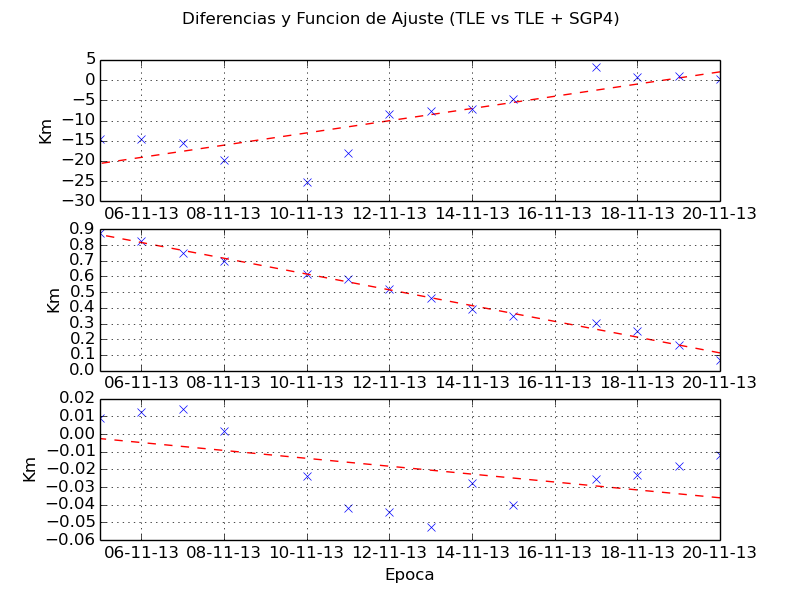
\includegraphics[width=0.7\linewidth]{imagenes/graf_2013pw.png}
  \caption{A subfigure}
  \label{fig:sub1}
\end{subfigure}%
\begin{subfigure}%{0.5\textwidth}
  \centering
  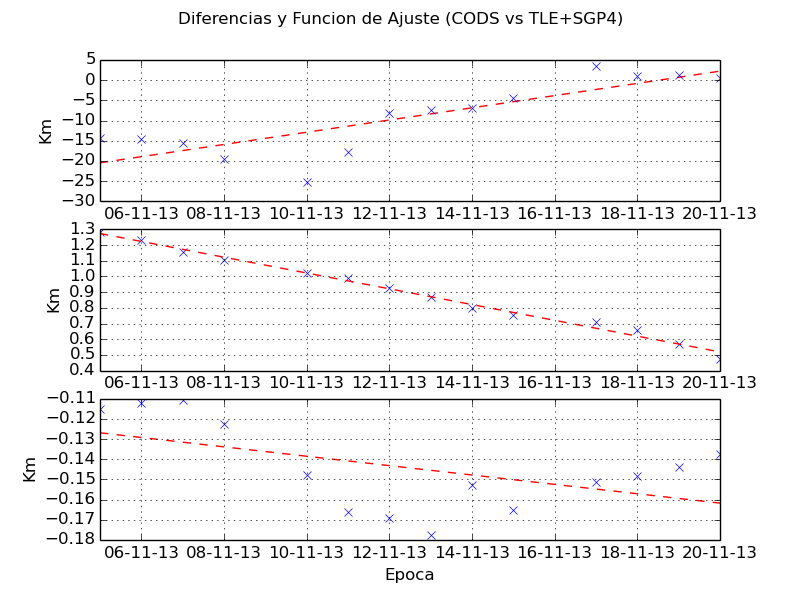
\includegraphics[width=0.7\linewidth]{imagenes/graf_codsOsweiler.png}
  \caption{A subfigure}
  \label{fig:sub2}
\end{subfigure}
\caption{A figure with two subfigures}
\label{fig:test}
\end{figure}



\subsubsection{Ma. de Covarianza Simplificada}
Se construye a partir de las diferencias entre las efem\'erides predichas por CODS y los vectores de estado que resultan de los TLEs.\\


\subsubsection{Ma. de Covarianza Ajustada}
Se construye a partir de las diferencias recalculadas a partir de los vectores de estado que resultan de los TLEs, corregidos por el ajuste.\\


\subsubsection{Procedimiento de Ajuste}
Consideramos la Misi\'on SAC-D.

Nos preguntamos:\\
\begin{equation}
 x_{TLE}-x_{cods} > ? (x_{TLE}-x_{e})-x_{i}
\end{equation}
\begin{itemize}
 \item $x_{TLE}$: Valor del vector de estado a partir del TLE.\\
 \item $x_{cods}$: Efem\'eride predicha por CODS.\\
 \item $x_{e}$: Valor extrapolado a partir de la funci\'on de ajuste.\\
 \item $x_{i}$: Efem\'eride iterpolada a la \'epoca del TLE del intervalo de extrapolaci\'on.\\
\end{itemize}


Contamos con acceso a los datos de las efem\'erides predichas calculadas por CODS, pero no están publicados en estos archivos los errores asociados al c\'alculo.\\
Nos proveemos de los TLE de la Misi\'on para la misma \'epoca.\\
Evaluamos las diferencias entre los distintos vectores de estado (el predico por CODS y el que resulta de TLE).\\

\begin{equation}
 \delta x = x_{TLE}-x_{cods}
\end{equation}


{\bf{M\'etodo para la estimaci\'on del error en los datos extrapolados.}}\\
Se definen dos intervalos: uno para el ajuste $t_{a}$, otro para la extrapolaci\'on $t_{e}$.\\
Se ajustan en forma lineal las diferencias y se obtiene una funci\'on de ajuste.\\
\begin{equation}
 f=a*t+b \qquad a,b\quad par\\'ametros\quad del \quad ajuste.
\end{equation}

Se eval\'ua la funci\'on de ajuste en las fechas correspondientes a los TLEs del intervalo de extrapolaci\'on.\\
\begin{equation}
 x_{e}=f(t_{e})
\end{equation}

{\textcolor{red}{Se interpolan los valores de CODS $x_{int}$ para las fechas de los TLE del intervalo de extrapolaci\'on.}}\\
Se corrigen los valores de los vectores de estado de los TLE del intervalo de extrapolaci\'on, utilizando los valores que ofrece la funci\'on de ajuste. (En este punto se pretende que las posiciones y velocidades de los TLEs se acerquen a las posiciones y velocidades que ofrece CODS.)\\
\begin{align}
 x&=x_{e}-f & \delta x_{i}& = x_{i} - x 
\end{align}


